\author{João Gonçalves}
\newcommand{\authorr}{Teresa Nogueira}
\newcommand{\authorrr}{André Teodósio}
\newcommand{\authorrrr}{Francisco Carvalho}
\newcommand{\studentID}{99995}
\newcommand{\studentIDD}{100029}
\newcommand{\studentIDDD}{99889}
\newcommand{\studentIDDDD}{99941}
%\newcommand{\supervisorone}{Prof\textsuperscript{\underline{a}}. XXXXXX}
\newcommand{\supervisorone}{João Silvestre}
\newcommand{\supervisortwo}{}
\newcommand{\department}{Engenharia Eletrotécnica e de Computadores}
\newcommand{\exam}{Modelação e Simulação}

\title{%
Trabalho 3\\
\large Bola saltitante}
\date{Janeiro 2023}

\documentclass[a4paper,12pt]{article}
\usepackage[left=28mm,top=25mm,right=28mm,bottom=24mm]{geometry}
\usepackage[flushmargin,hang,bottom,multiple]{footmisc}
\usepackage{etoolbox}
\usepackage{pgfplots}
\usepackage{circuitikz}
\usepackage{booktabs}
\usepackage[usestackEOL]{stackengine}
\usepackage[T1]{fontenc}
\usepackage[utf8]{inputenc}
\usepackage{bm}
\usepackage[export]{adjustbox}
\usepackage{graphicx}
\usepackage[font=footnotesize]{caption}
\usepackage[justification=centering]{subcaption}
\usepackage{amsmath}
\usepackage{amsfonts}
\usepackage{mathtools}
\usepackage{float}
\usepackage[linktoc=all]{hyperref}
\usepackage[capitalise]{cleveref}
\usepackage{enumitem,kantlipsum}
\usepackage[square,numbers,sort]{natbib}
\usepackage[ruled,vlined]{algorithm2e}
\usepackage{listings}
\usepackage[numbered,framed]{matlab-prettifier}
\usepackage{minted}
\usepackage{amssymb}
\usepackage{babel}
\usepackage[nottoc,numbib]{tocbibind}
\usepackage{tcolorbox}
\usepackage{xcolor}
\usepackage{graphicx,array}
\usepackage{animate}
\usepackage{breakurl}
\usepackage{placeins}
\usepackage{colortbl}
\usepackage{attrib}
\usepackage{wrapfig}
\usepackage{mathabx}
\usepackage{fancyhdr}
\usepackage{amsmath}
\usepackage{lipsum}
\usepackage{textcomp}
\usepackage[framemethod=TikZ]{mdframed}
%\tcbuselibrary{skins,breakable}
%\usetikzlibrary{shadings,shadows}
\usemintedstyle{emacs}
\linespread{1}
%\setlength{\parindent}{0pt}

\usepackage{multimedia}

\newenvironment{block}[1]{%
    \tcolorbox[beamer,%
    noparskip,breakable,
    colback=LightBlue,colframe=DarkBlue,%
    colbacklower=DarkBlue!75!LightBlue,%
    title=#1]}%
    {\endtcolorbox}

\hypersetup{
    colorlinks,
    linkcolor={black},
    citecolor={blue!50!black},
    urlcolor={blue!80!black}
}

\lstset{
  style              = Matlab-editor,
  basicstyle         = \scriptsize\mlttfamily,
  escapechar         = ",
  mlshowsectionrules = true,
  extendedchars=true,
  literate= {á}{{\'a}}1 {é}{{\'e}}1 {í}{{\'i}}1 {ó}{{\'o}}1 {ú}{{\'u}}1 {ç}{{\c c}}1 {ã}{{\~a}}1 {õ}{{\~o}}1
  {Á}{{\'A}}1 {É}{{\'E}}1 {Í}{{\'I}}1 {Ó}{{\'O}}1 {Ú}{{\'U}}1 {Ã}{{\~A}}1,
}

%//==============================--@--==============================//%
%                         -> error messages <-                        %
\usepackage{pifont,mdframed}

\newenvironment{warning}
  {\par\begin{mdframed}[linewidth=1.5pt,linecolor=red]%
    \begin{list}{}{\leftmargin=0.9cm
                   \labelwidth=\leftmargin}\item[\raisebox{-0.4 em}{\Large\ding{43}}]}
  {\end{list}\end{mdframed}\par}

%//==============================--@--==============================//%
%                   -> reduzir espaço entre itens <-                  %
\usepackage{enumitem}
%\setlist[itemize]{nosep}
%\setlist[enumerate]{nosep}
\setlist[itemize]{itemsep=0.0125em}
\setlist[enumerate]{itemsep=0.0125em}
%//==============================METH-==============================//%
\newcounter{theo}[section]\setcounter{theo}{0}
\renewcommand{\thetheo}{\arabic{theo}}

\definecolor{tempcolor}{RGB}{113, 110, 97}
\newenvironment{theo}[2][]{%
    \refstepcounter{theo}
    \ifstrempty{#1}%
    % if condition (without title)
    {\mdfsetup{%
        frametitle={%
            \tikz[baseline=(current bounding box.east),outer sep=0pt]
            \node[anchor=east,rectangle,fill=blue!20]
            {\strut Teorema~\thetheo};}
        }%
    % else condition (with title)
    }{\mdfsetup{%
        frametitle={%
            \tikz[baseline=(current bounding box.east),outer sep=0pt]
            \node[anchor=east,rectangle,fill=black!20]
            {\strut #1};}%
        }%
    }%
    % Both conditions
    \mdfsetup{%
        innertopmargin=0pt,linecolor=tempcolor,%
        linewidth=2pt,topline=true,%
        frametitleaboveskip=\dimexpr-\ht\strutbox\relax%
    }
 
\begin{mdframed}[]\relax}{%
\end{mdframed}}

\def\delequal{\mathrel{\ensurestackMath{\stackon[1pt]{=}{\scriptstyle\Delta}}}}
%------------------------------------ MAGIC--------------------------------------
\def\UrlBreaks{\do\/\do-}
\expandafter\def\expandafter\UrlBreaks\expandafter{\UrlBreaks\do\a%
\do\b\do\c\do\d\do\e\do\f\do\g\do\h\do\i\do\j\do\k\do\l\do\m\do\n%
\do\o\do\p\do\q\do\r\do\s\do\t\do\u\do\v\do\w\do\x\do\y\do\z\do\&}

\newcolumntype{C}[1]{>{\centering\let\newline\\\arraybackslash\hspace{0pt}}m{#1}}
\newcolumntype{L}[1]{>{\raggedright\let\newline\\\arraybackslash\hspace{0pt}}m{#1}}
%----------------------------------TITLE PAGE -----------------------------------
\makeatletter
\def\maketitle{
  \begin{center}\leavevmode
        \normalfont
        
\includegraphics[width=0.5\columnwidth]{img/title-page/IST.pdf}
        \vskip 0.05cm   
        \textsc{\large \department}\\
        \vskip 0.5cm
        \rule{0.95\linewidth}{0.2 mm} %\\
        {\large \exam}\\[0.5 cm]
        {\huge \bfseries \@title \par} 
        \vspace{0.5em}
        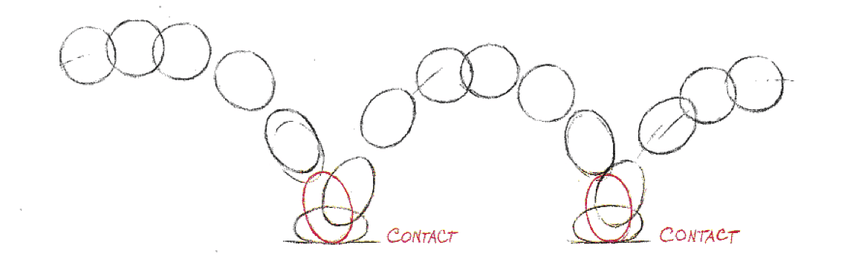
\includegraphics[scale=0.35]{img/title-page/000.png}
        \vspace{-0.5em}
        \captionof*{figure}{\color{gray} Imagem: Bouncing ball (Roberts \& Mallet 2013)}
        %\vspace{0.5cm}
        \rule{0.95\linewidth}{0.2 mm} \\[0.75 cm]
        %\fontsize{9pt}{11pt}\selectfont
        \begin{minipage}[t]{0.45\textwidth}
	    \begin{flushleft} \large
                \emph{Autores:}\\
		    \normalsize \textbf{\authorrr} : \studentIDDD\\
                \scriptsize $\hookrightarrow$ andre.teodosio@tecnico.ulisboa.pt \\
                \normalsize \textbf{\authorrrr} : \studentIDDDD \\
                \scriptsize $\hookrightarrow$ franciscosoaresc@tecnico.ulisboa.pt
            \end{flushleft}
	\end{minipage}
        \begin{minipage}[t]{0.45\textwidth}
	   \begin{flushleft} \large
                \vphantom{teste 123} \\
			\normalsize \textbf{\@author} : \studentID\\
                \fontsize{9pt}{11pt}\selectfont $\hookrightarrow$ jrazevedogoncalves@tecnico.ulisboa.pt \\
                \normalsize \textbf{\authorr} : \studentIDD\\
                \scriptsize $\hookrightarrow$ maria.teresa.ramos.nogueira@tecnico.ulisboa.pt
		\end{flushleft}
	\end{minipage}
        \vskip 1em
        \begin{minipage}[t]{0.45\textwidth}
	   \begin{flushleft} \large
			\ifdefempty{\supervisortwo}{\emph{Docente:\\}}{\emph{Docentes:\\}}
			\supervisorone\\
			\ifdefempty{\supervisortwo}{}{\supervisortwo\\}
		\end{flushleft}
	\end{minipage}
         \begin{minipage}[t]{0.45\textwidth}
	   \begin{flushright} \large
			\phantom{123 experiência}
		\end{flushright}
	\end{minipage}
        \vspace{0.35cm}
        \begin{quotation}
            \textit{O grupo de alunos acima identificado garante que o texto deste relatório e todo o software e resultados entregues foram inteiramente realizados pelos elementos do grupo, com uma participação significativa de todos eles, e que nenhuma parte do trabalho ou do software e resultados apresentados foi obtida a partir de outras pessoas ou fontes.}
        \end{quotation}
	\vfill
	{\Large \@date\par}
   \end{center}
   %\vfill
   %\null
   \cleardoublepage
  }
\makeatother
%-------------------------------- ENDTITLE PAGE ----------------------------------
%---> Header <---
%\fancyhf{}
\renewcommand{\headrulewidth}{1pt}% Header rule width
\renewcommand{\footrulewidth}{0pt}% No footer rule
\setlength\headheight{26pt} 
\fancyhead[L]{\raisebox{0.1\height}[0pt][0pt]{\textit{Modelação e Simulação}}}
\fancyhead[R]{\raisebox{0.1\height}[0pt][0pt]{2022/2023}}

\pgfplotsset{compat=1.18}
\setcounter{tocdepth}{4}
%\setcounter{secnumdepth}{4}
\setcounter{secnumdepth}{-2}

\renewcommand{\figurename}{Fig.}
\renewcommand{\tablename}{Tab.}
\renewcommand{\contentsname}{Índice}
\settocbibname{\raisebox{4em}{Referências}}
\setlength{\bibsep}{0.1em}%reduzir espaço entre refs.

\renewcommand{\bibpreamble}{\vspace{-8em}}

\begin{document}
    \sloppy
    %% title page
    \pagenumbering{gobble}
    \maketitle
    %% toc
    %\tableofcontents
    %% body
    \newpage
    \pagestyle{fancy}
    \pagenumbering{arabic}
    %\phantomsection\addcontentsline{toc}{section}{}\vskip -0em%
        \usetikzlibrary{automata, arrows.meta, positioning}
%//==============================--@--==============================//%
%\vspace{-1em}
\section{Introdução}
\label{sec:intro}

Uma vasta panóplia de sistemas mecânicos envolvem \underline{impactos}. Estes sistemas admitem um \textit{flow}\footnotemark[1] entre impactos. A aproximação (amplamente) considerada para os impactos sugere considerá-los como instantâneos---e, consequentemente, como \textit{triggers} que levam a transições de estado do sistema (\textit{jumps}\footnotemark[1]). 

Deste modo, \underline{sistemas com impactos}---tal como o caso de estudo---podem ser vistos como \underline{sistemas híbridos}.

%//==============================--A--==============================//%
\vspace{1em}
\noindent $\pmb{\rightarrow}$ \textit{\textbf{Bola saltitante} (modelo de massa puntiforme---lagrangian hybrid system)}
\vspace{0.25em}

\noindent O estado da massa pontual pode ser descrito como

\vspace{-0.9em}
$$
    \pmb{x} := 
            \begin{bmatrix}
                z\\
                v_z
            \end{bmatrix}
            \in \mathbb{R}_{\ge 0} \times \mathbb{R}
            \text{,}
$$

\vspace{-0.2em}
\noindent onde $z$ representa a posição da bola (acima da superfície), e $v_z$ a velocidade vertical.

É natural estipular que o \textit{flow} é permissível quando a bola se encontra acima da superfície, ou quando se encontra na superfície com o vetor velocidade a apontar para cima. Deste modo, o \textit{flow set} é

\vspace{-1em}
$$ 
    C := \left\{ \pmb{x}: z > 0\; \lor\; z = 0\; \land\; v_z \ge 0 \right\}.
$$

\vspace{-0.25em}
\noindent E a escolha do \textit{flow map} pode ser dada por

\vspace{-0.75em}
$$
    f(\pmb{x}) := \begin{bmatrix} v_z \\ -g \end{bmatrix}\qquad \forall \pmb{x} \in C\text{,}
$$

\vspace{0em}
\noindent onde $-g$ representa a aceleração gravítica. Os impactos sucedem-se com o embate da massa pontual com velocidade negativa com a superfície. E assim, o \textit{jump set}\footnotemark[2] é

\vspace{-1em}
$$
    D := \left\{ \pmb{x}: z = 0,\; v_z < 0 \right\}.
$$

\vspace{-0.25em}
\noindent O \textit{jump map} é dado, para um determinado $\alpha \in [0, 1]$ (coeficiente de restituição), por

\vspace{-0.75em}
$$
    g(\pmb{x}) := \begin{bmatrix} 0 \\ -\alpha\,v_z \end{bmatrix} \quad \forall \pmb{x} \in D\text{.}
$$
\vspace{-1.75em}
\begin{figure}[H]
    \begin{minipage}[c]{0.4\linewidth}
        \begin{tikzpicture}[node distance = 2.7cm, on grid, auto, transform shape]
            
            \node[state,
                initial,
                initial text = {$\pmb{x}(t_0) \in C$},
                fill=orange!20,
                align=center,
                inner sep=0pt] (q_0) 
            {\textit{\underline{Flow}}\\ $\begin{cases} \dot{z} = v_z\\ \dot{v_z} = -g \end{cases}$\\ $\pmb{x} \in C$};
            
            \path [-stealth, thick]
                (q_0) edge[loop right] 
                node[above, yshift = 0.5cm]
                    {$\pmb{x} \in D$}
                node[right, yshift = -0.25cm] 
                    {$\begin{aligned}
                        &\;\, \textit{\underline{Jump}}\\[-0.7ex]
                        v_z &:= -\alpha \cdot v_z
                    \end{aligned}$} 
                (q_0);
                
        \end{tikzpicture}
    \end{minipage}\hfill
    \begin{minipage}[c]{0.45\linewidth}
    $$
        \:\pmb{\iff}\;\:
        \begin{cases}
            \pmb{x} \in C & \dot{\pmb{x}} = f(\pmb{x}) \\
            \pmb{x} \in D & \pmb{x}^{+} = g(\pmb{x}) 
        \end{cases}
    $$
    \end{minipage}
    \caption{\underline{Modelo da bola saltitante}.}
    \label{fig:bouncing-ball}
\end{figure}

\vspace{-0.75em}
\noindent No \hyperref[fig:bouncing-ball]{modelo para a bola saltitante exposto acima}, para um $\alpha \in\, ]0,1[$, cada \textit{jump} é seguido por um período de \textit{flow} (sucessivamente mais curto). Por outras palavras, \textit{jumps} consecutivos não ocorrem\cite{Goebel2012-ho} (apesar de se verificarem consecutivamente menos espaçados, $\to 0$). Estas ilações iluminam o \hyperref[def:zeno]{\underline{efeito de Zeno}}, também alvo de estudo.

\begin{theo}[\underline{Def.:} Efeito de Zeno $\pmb{\star}$]{def:zeno}
    \label{def:zeno}
    ``\textit{Zeno behavior is a phenomenon in hybrid systems that (...) exists when an \underline{infinite number of discrete transitions occur in a finite time interval}}.''\cite{Ames2006-fl}
\end{theo}

%//==============================--@--==============================//%
\footnotetext[1]{``\textit{To shorten the terminology, the behavior of a dynamical system that can
be described by a differential equation or inclusion is referred to as flow. The behavior of a dynamical system that can be described by a difference equation or inclusion is referred to as jumps}.''\cite{Goebel2012-ho}}
\footnotetext[2]{Devido ao funcionamento do SIMULINK\textregistered{} consideramos, na simulação computacional, um $z \le 0$.}
    \phantomsection\addcontentsline{toc}{section}{Perguntas}\vskip -0em%
        \clearpage

\def\testeimplies{\mathrel{\ensurestackMath{\stackon[1pt]{\implies}{\scriptstyle t_0 \equiv 0}}}}
\def\testeimpliess{\mathrel{\ensurestackMath{\stackon[1pt]{\implies}{\scriptstyle v_z(t_1^-) < 0}}}}
%//==============================--@--==============================//%
%\vspace{-1em}
\subsection{P1 | Simulação do movimento da bola (somente na vertical)}
\label{subsec:P1}

De modo a caracterizar as condições \underline{base} de partida que fomentam o estudo dos efeitos do coeficiente de restituição $\alpha$, e da velocidade inicial $v_z(t_0^+)$, apresentam-se abaixo, na \hyperref[fig:P1-SistemaCompleto]{Fig. 2}, a evolução temporal da posição da bola saltitante e da sua velocidade vertical para $z(t_0) := z_0 = 10$ m, $v_{z}(t_0^+) := v_{z_0} = 0$ ms$^{-1}$ e $\alpha = 0.8$. 

\begin{wrapfigure}[14]{l}{0.575\textwidth}
    \centering
    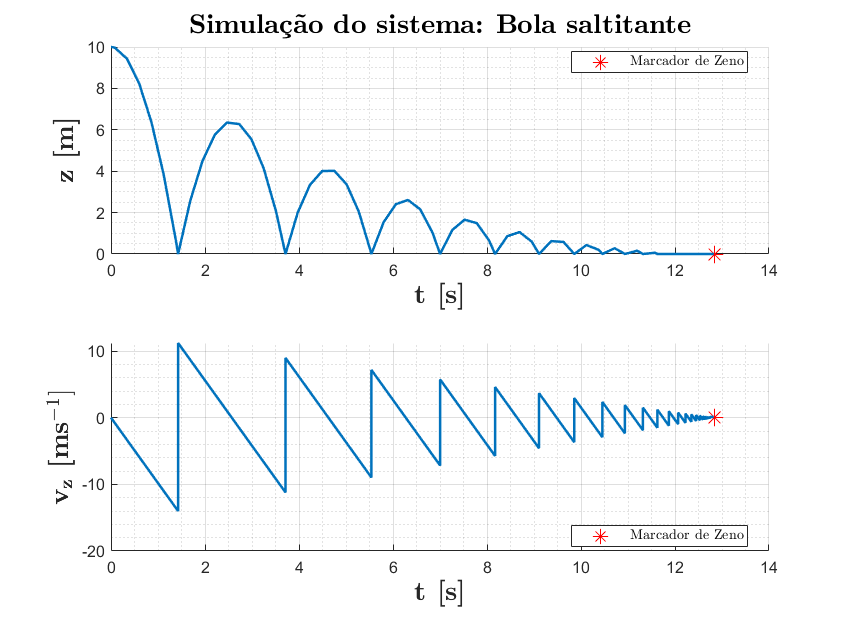
\includegraphics[width=0.575\textwidth]{img/P1/P1-SistemaCompleto.png}
    \caption{Simulação do sistema para as condições iniciais supramencionadas e $\alpha = 0.8$ ($t_0 \equiv 0$).}
    \label{fig:P1-SistemaCompleto}
\end{wrapfigure}

\vphantom{123}

\noindent\textbf{\textit{$\rightarrow$ Observações}}
\vspace{-0.5em}
\begin{itemize}
    \item[$\blacktriangle$] Verifica-se a descontinuida- de da velocidade no instan- te de embate da bola com a superfície (\textit{jump})\protect\footnotemark[3].
    
    \item[$\blacktriangle$] Afunilamento sucessivo ex- pectável da velocidade com base nas perdas energéticas.
    
    \item[$\blacktriangle$] A bola saltitante é incapaz de atingir a posição vertical inicial graças à dissipação energética imposta pelo fator $\alpha = 0.8$.
\end{itemize}

\footnotetext[3]{Denota-se a velocidade logo antes e após o choque com os $-$ e $+$ sobrescritos, respetivamente.}

\vspace{1em}
\noindent A posição vertical da massa pontual em períodos de \textit{flow} é regida pela equação:
\vspace{-0.5em}
$$
    z(t + t_{n-1}) = z(t_{n-1}) + v_{z}(t_{n-1}^+) \cdot t - \frac{1}{2}g \cdot t^2\qquad n = 1, 2, \dots
$$

\vspace{-0.5em}
\noindent em que $z(t_{n-1})$ é a altura inicial do período de \textit{flow}\footnotemark[4] $n$, e $v_{z}(t_{n-1}^+)$ a velocidade inicial desse mesmo período (para $n \ge 2$, será a velocidade após o \textit{jump} \hyperref[sec:intro]{definido acima}).

\footnotetext[4]{A altura inicial é nula para todos os períodos de \textit{flow} subsequentes ao 1\textordmasculine{} ($n \ge 2: z(t_{n-1}) \equiv 0$). Para o primeiro período ($n=1$), são assumidas as condições iniciais impostas: $z_0$ e $v_{z_0}$.}

Relembrando a \underline{Lei de Conservação d'Energia}: $\Delta E = \Delta T + \Delta U = 0$ (dado que não são aplicadas forças externas ao sistemas ao longo de cada período de \textit{flow}), trivialmente se obtém $v_{z}$ imediatamente antes do primeiro choque:
\vspace{-0.5em}
$$
    \Delta E = 0 \iff mg z_0 + \frac{1}{2}m (v_{z_0})^2 = \frac{1}{2}m [v_{z}(t_{1}^-)]^2 \:\testeimpliess\: v_z(t_{1}^-) = -\sqrt{2 g z_0 + (v_{z_0})^2}
$$

\vspace{-0.5em}
\noindent Para condições iniciais arbitrárias, o tempo acumulado após $N$ choques é dado por:

\vspace{-0.5em}
$$
    T_N = t_1 + t_2 + t_3 + \dots = \frac{v_{z_0}}{g} +  \frac{\sqrt{2 g z_0 + (v_{z_0})^2}}{g} \left(1 + 2 \sum\limits_{n=1}^{N-1} \alpha^n \right)
$$
em que $t_n$ representa a duração\footnotemark[5] do $n$-ésimo período de \textit{flow}, para $n \in \mathbb{N}$.

A série geométrica com razão $\alpha$, converge para valores do coeficiente $\alpha \in [0,\,1[$. Define-se finalmente o tempo em que ocorre o \hyperref[def:zeno]{fenómeno de Zeno}\footnotemark[9]\footnotemark[10]:
\vspace{-0.5em}
$$
    \therefore T_{Zeno} := \lim\limits_{N \to +\infty} T_N = \frac{1}{g} \left(v_{z_0} + \sqrt{2 g z_0 + (v_{z_0})^2} \left(\frac{1+\alpha}{1-\alpha}\right)\right),\quad \alpha \in [0,\,1[
$$

\vspace{-0.5em}
\noindent \textbf{Nota} $\pmb{\rightarrow}$ Conceptualmente, $T_{Zeno}$ pode ser visto como o tempo \underline{teórico} necessário até que ``\textit{(...) the ball settles down to the ground with zero velocity (...)}''\cite{mathworks-bouncingball}.

\footnotetext[5]{Note-se que $t_n$ é a solução positiva da equação quadrática $z(t+t_{n-1}) = 0$, para $n = 1, 2, \dots$ ($t_0 \equiv 0$).}
%//==============================--C--==============================//%
\clearpage

\noindent $\pmb{\rightarrow}$ \textbf{\textit{Condições iniciais e fenómeno de Zeno}}

\noindent Para as condições iniciais \hyperref[fig:P1-SistemaCompleto]{expostas acima} e $\alpha = 0.8$, obtém-se $T_{Zeno} = 12.8506\text{ s}$. Este fenómeno é capturado em ambiente de simulação através da deteção (\textit{default}) de \textit{consecutive zero crossing events} em intervalos de tempo ínfimos:

\begin{warning}
    \footnotesize\color{red}\texttt{An error occurred while running the simulation (...): Simulink will stop the simulation of model 'P1simulink' because the 1 zero crossing signal(s) identified below caused 1000 consecutive zero crossing events in time interval between 12.850588106411884 and 12.850588107006466.}
\end{warning}

\vspace{-0.5em}
\noindent Na \hyperref[fig:P1-SistemaCompleto]{Fig. 2 acima}, este comportamento é delimitado pelo "marcador de Zeno" ({\color{red} $\star$}).

De modo a garantir a generalidade da discussão, explora-se a (expectável) relação íntima entre o fator de atenuação e da velocidade inicial com o valor de $T_{Zeno}$. 

%\setcounter{footnote}{0}
%\renewcommand*{\thefootnote}{\fnsymbol{footnote}}
\vspace{-0.75em}
\begin{figure}[H] 
    \begin{subfigure}[b]{0.33\linewidth}
        \centering
        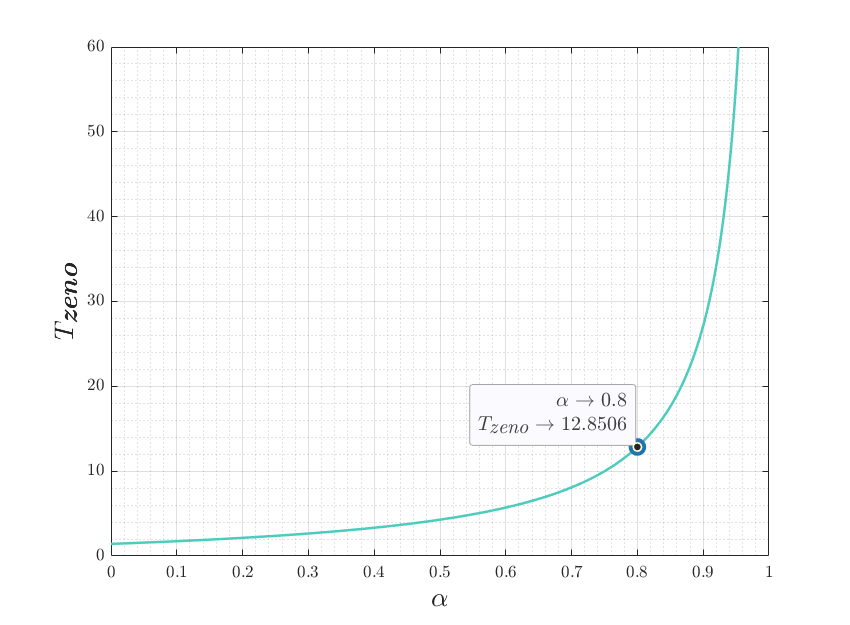
\includegraphics[width=1\linewidth]{img/P1/P1-coefTimpacto.png}
        \caption{$T_{Zeno}$: variação de $\alpha$ para $z_0 = 10$ m e $v_{z_0} = 0$ ms$^{-1}$} 
        \label{fig:coefTimpacto} 
    \end{subfigure}%% 
    \begin{subfigure}[b]{0.33\linewidth}
        \centering
        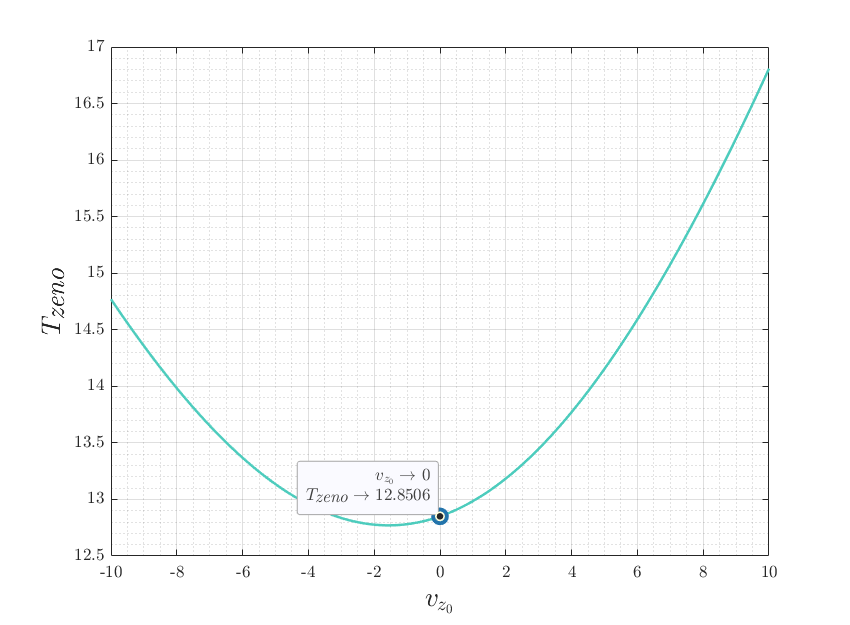
\includegraphics[width=1\linewidth]{img/P1/P1-veloTinf.png} 
        \caption{$T_{Zeno}$: variação de $v_{z_0}$ para $z_0 = 10$ m e $\alpha = 0.8$} 
        \label{fig:veloTinf} 
    \end{subfigure}
    \begin{subfigure}[b]{0.33\linewidth}
        \centering
        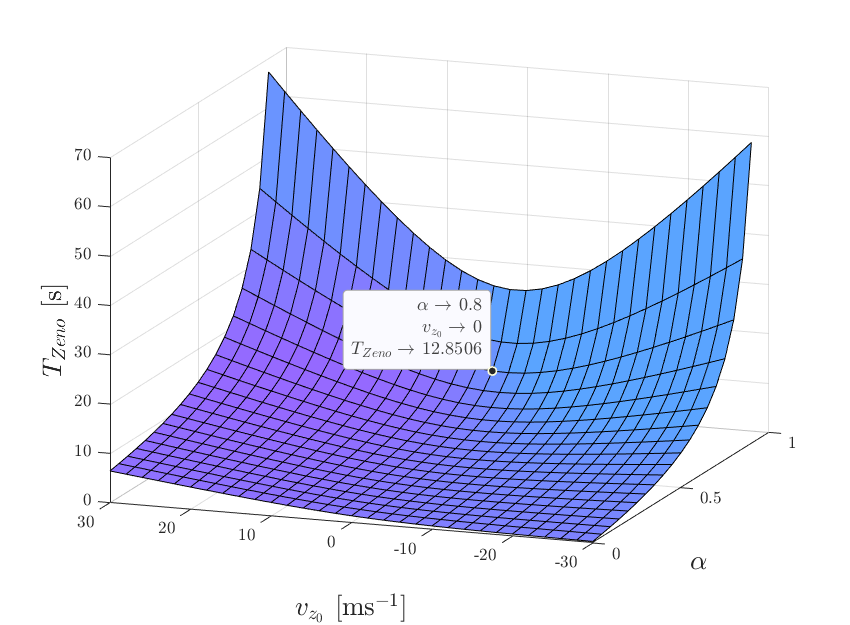
\includegraphics[width=1\linewidth]{img/P1/P1-3dplot.png} 
        \caption{$T_{Zeno}$: variação de $v_{z_0}$ e de $\alpha$, para $z_0 = 10$ m} 
        \label{fig:3dplot} 
    \end{subfigure} 
    \caption{Efeito da variação de $\alpha$ e $v_{z_0}$ no valor de $T_{Zeno}$. Note-se que, naturalmente, uma diminuição de $\alpha$ traduz-se numa diminuição de $T_{Zeno}$, e vice-versa\protect\footnotemark[6] (\textit{vide} \hyperref[fig:phase-portrait-limites]{Fig. 6}) $\rightarrow$ comportamento de acordo com a dinâmica energética do sistema imposta por este parâmetro. Curiosamente, verifica-se que ao alterar a energia inicial do sistema, impondo uma velocidade inicial (para um $\alpha \in\, ]0,\, 1[$), despoleta uma evolução de $T_{Zeno}$---não óbvia---visível na \hyperref[fig:veloTinf]{curva (b)}. Verifica-se que o valor de $v_{z_0}$ que minimiza $T_{Zeno}$, para um determinado $\alpha$ fixo (e $z_0 \in \mathbb{R}_{>0}$), é sempre inferior a $0$\protect\renewcommand*{\thefootnote}{\fnsymbol{footnote}}\protect\footnotemark[2] (\hyperref[fig:Derivada]{Fig. 4 (a)}).}
\end{figure}

\renewcommand*{\thefootnote}{\arabic{footnote}}
\footnotetext[6]{Do outro lado do espectro, um $\alpha \to 1$ implica um aumento avassalador de $T_{Zeno}$ ($\to +\infty$), como aparente na \hyperref[fig:matrixcoef]{Fig. 4 (c)} e nos \hyperref[fig:phase-portrait]{retratos de fase subsequentes}.}

\footnotetext[7]{O $v_{z_0}$ minimizante de $T_{Zeno}$ diminui o intervalo de tempo até ao 1\textordmasculine{} choque, não aumentando substancialmente os períodos de \textit{flow} subsequentes.}

\renewcommand*{\thefootnote}{\fnsymbol{footnote}}
\footnotetext[2]{ 
$
    \left.\dfrac{\partial T_{Zeno}}{\partial v_{z_0}}\right\vert_{\alpha} = 
    \dfrac{1}{g}\left(\cfrac{v_{z_0}}{\sqrt{2 g z_0 + (v_{z_0})^2}}\left(\dfrac{1+\alpha}{1-\alpha}\right)+1\right) =
    0
    \implies
    v_{z_0}\biggr\rvert_{\alpha} = -\sqrt{\dfrac{g z_0 \left( 1-\alpha \right)^2}{2\alpha}}
$ \hfill\raisebox{-0.8 em}{\ensuremath{\Box}}
}

%\noindent experiência %sim adoro-te :3
\vspace{-1em}
\noindent Como lembra a Análise Matemática, o valor de $v_{z_0}$ que minimiza $T_{Zeno}$ (mínimo local) para um dado $\alpha$, é deduzido através da 1\textordfeminine{} derivada parcial em ordem a $v_{z_0}$\footnotemark[2]$\mkern-1mu^{,}$\renewcommand*{\thefootnote}{\arabic{footnote}}\footnotemark[7].

\renewcommand*{\thefootnote}{\fnsymbol{footnote}}

\vspace{-0.75em}
\begin{figure}[ht] 
     \begin{subfigure}[b]{0.33\linewidth}
        \centering
        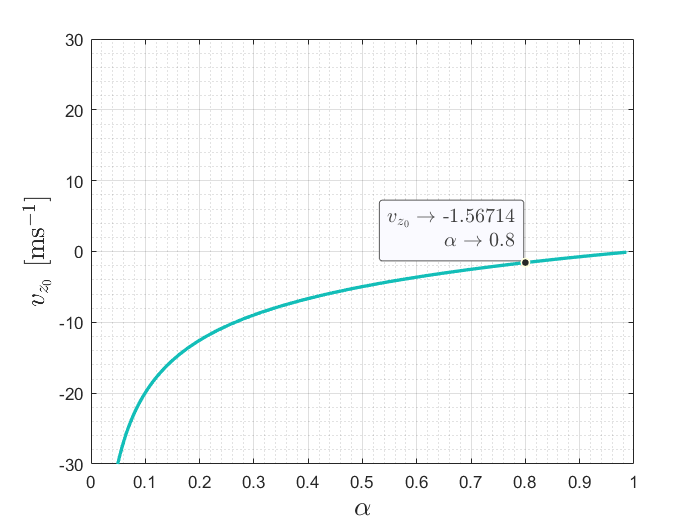
\includegraphics[width=1\linewidth]{img/P1/P1-DerivadaShenanigan.png} 
        \caption{$(\partial T_{Zeno}/\partial v_{z_0})|_{\alpha} = 0 $\protect\footnotemark[2]\\ \vphantom{}} 
        \label{fig:Derivada} 
    \end{subfigure}%%
    \begin{subfigure}[b]{0.33\linewidth}
        \centering
        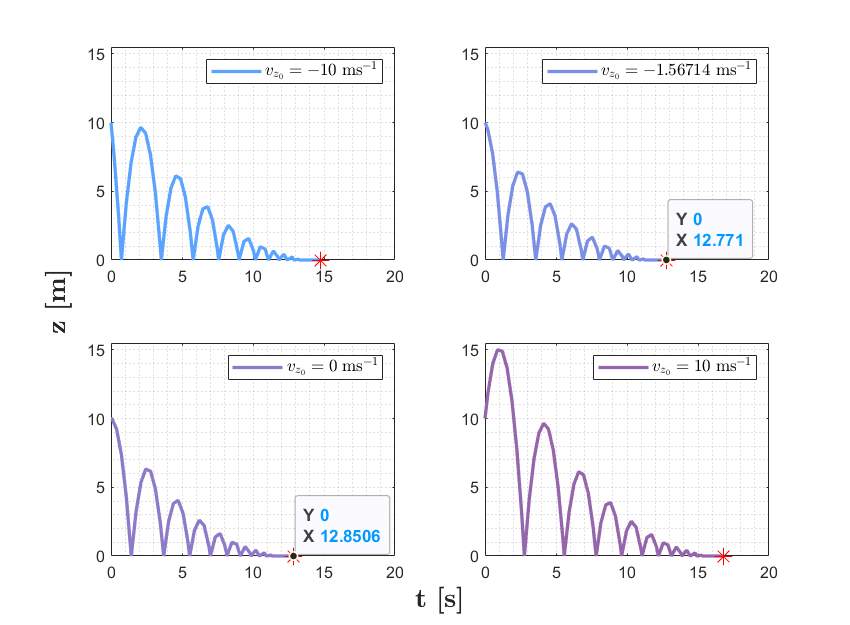
\includegraphics[width=1\linewidth]{img/P1/P1-velomatrix.png} 
        \caption{Posição vertical da bola para $v_{z_0}$ variável ($\alpha = 0.8$).} 
        \label{fig:matrixvelo} 
    \end{subfigure}%%
    \begin{subfigure}[b]{0.33\linewidth}
        \centering
        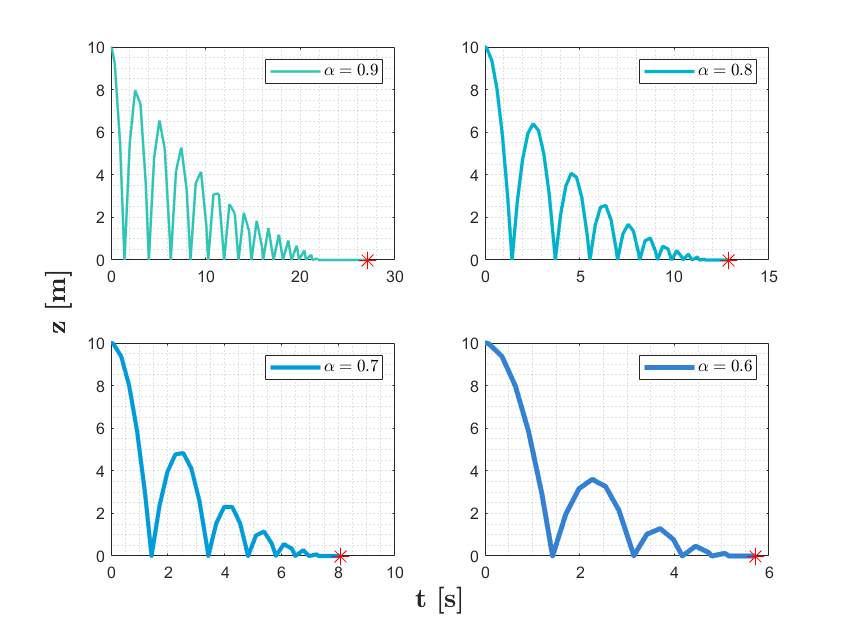
\includegraphics[width=1\linewidth]{img/P1/P1-coefmatrix.png}
        \caption{Posição vertical da bola para $\alpha$ variável ($v_{z_0} = 0$ ms$^{-1}$).} 
        \label{fig:matrixcoef} 
    \end{subfigure}%%
    \caption{Curva de nível da derivada parcial de $T_{Zeno}$ em ordem a $v_{z_0}$\protect\footnotemark[2] e visualização temporal da posição vertical da massa puntiforme relativamente a alguns exemplos que espelham o efeito da variação da velocidade inicial e do fator de atenuação (para um $z_0 = 10$ m).}
\end{figure}

%\setcounter{footnote}{4}
\renewcommand*{\thefootnote}{\arabic{footnote}}

%//==============================--A--==============================//%
\clearpage
\noindent $\pmb{\rightarrow}$ \textbf{\textit{Retratos de fase}}

\noindent O efeito do coeficiente de restituição $\alpha$ e de $v_{z_0}$ são apresentados condensadamente através da visualização dos retratos de fase do sistema. Note-se: para valores de $\alpha\in [0,\, 1[$ ocorre uma diminuição (expectável) da velocidade vertical após cada impacto e consequentemente da altura máxima\footnotemark[8] atingida pela massa pontual no período de \textit{flow} que sucede o embate com a superfície horizontal. Este fenómeno é cada vez mais acentuado para valores de $\alpha$ sucessivamente mais próximos de $0$ (\textit{vide} \hyperref[fig:phase-portrait-limites]{Fig. 6}).

\footnotetext[8]{Denominaremos por $z_\textit{máx}$ este valor daqui em diante.}

\vspace{-0.65em}
\begin{figure}[H]
    \centering
    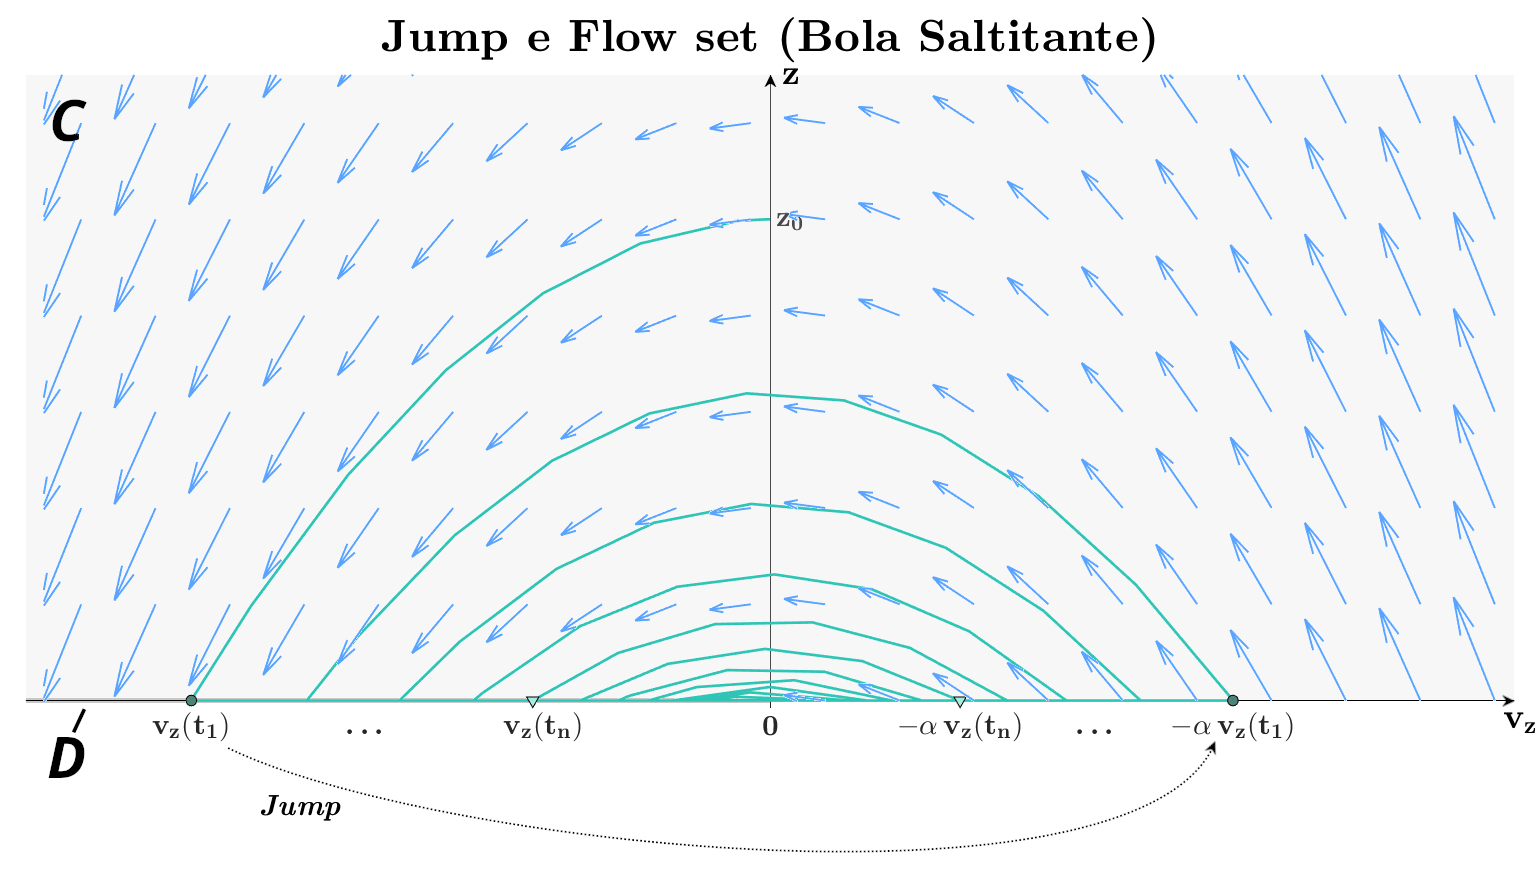
\includegraphics[width = 0.9\linewidth]{img/P1/P1-PhasePortrait.png}
    \caption{Retrato de fase do sistema para $z_0 = 10$ m, $v_{z_0} = 0$ ms$^{-1}$ e $\alpha = 0.8$. (Exemplo que traduz a resposta para valores de $\alpha \in\, ]0,\, 1[$ $\rightarrow$ \textbf{colisões elásticas}\protect\footnotemark[9] $\rightarrow$ perdas energéticas com o embate na superfície; salienta-se a diminuição dos intervalos entre colisões---resposta naturalmente esperada para o caso exposto, cada vez mais acentuada para valores de $\alpha$ cada vez mais pequenos).}
    \label{fig:phase-portrait}
\end{figure}

\footnotetext[9]{``\textit{It is easily shown that if the impacts are not perfectly elastic, the ball displays Zeno behavior}''\cite{Or2011-db}.}

\vspace{-1.25em}
\begin{figure}[ht] 
    \begin{subfigure}[b]{0.5\linewidth}
        \centering
        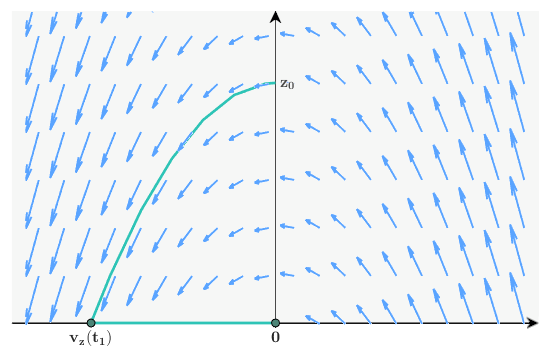
\includegraphics[width=1\linewidth]{img/P1/P1-PhasePortrait-alpha=0.png}
        \caption{Retrato de fase para $z_0 = 10$ m, $v_{z_0} = 0$ ms$^{-1}$ e\\ $\pmb{\underline{\alpha = 0}}$.} 
        \label{fig:phase-portrait-alpha0} 
    \end{subfigure}%% 
    \begin{subfigure}[b]{0.5\linewidth}
        \centering
        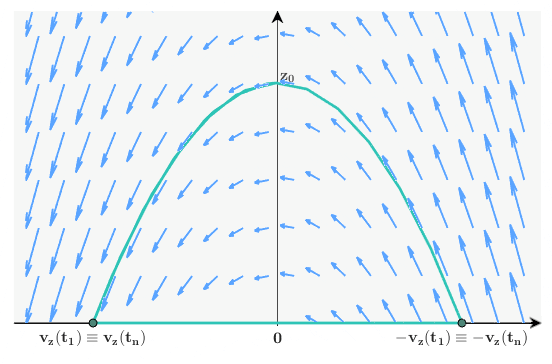
\includegraphics[width=1\linewidth]{img/P1/P1-PhasePortrait-alpha=1.png} 
        \caption{Retrato de fase para $z_0 = 10$ m, $v_{z_0} = 0$ ms$^{-1}$ e\\ $\pmb{\underline{\alpha = 1}}$.} 
        \label{fig:phase-portrait-alpha1} 
    \end{subfigure} 
    \caption{Comportamento do sistema da bola saltitante para os casos limites em que o coeficiente de restituição $\alpha$ toma os valores: $\pmb{0}$ (\textbf{colisão inelástica} $\rightarrow$ perda máxima de energia $\rightarrow \pmb{T_{Zeno} = t_1}$) e $\pmb{1}$ (\textbf{colisão perfeitamente elástica} $\rightarrow$ conservação total da energia cinética $\rightarrow \pmb{T_{Zeno} \to +\infty}$).}
    \label{fig:phase-portrait-limites}
\end{figure}

\vspace{-1em}
\noindent Acresce-se ainda o reparo: para $\alpha = 0$ existe somente um período de \textit{flow}\footnotemark[10] dado que toda a energia cinética é perdida com o choque e a massa pontual permanece, deste modo, pegada à superfície; para $\alpha = 1$ o comportamento repete-se \textit{ad aeternum}\footnotemark[10].

\footnotetext[10]{Para os casos limites $\alpha \in \{0, 1\}$, não se verifica o efeito de Zeno (\textit{vide} \hyperref[def:zeno]{secção introdutória}).}
%//==============================--@--==============================//%
        \clearpage
%//==============================--@--==============================//%
%\vspace{-1em}
\subsection{P2 | Perdas por atrito viscoso (proporcional à velocidade)}
\label{subsec:P2}

\begin{theo}[\underline{Def.:} Atrito Viscoso (\textit{drag}) $\pmb{\star}$]{def:zeno}
    \label{def:atrito}
    ``\textit{The force on an object that resists its motion through a fluid is called drag. When the fluid is a gas like air, it is called aerodynamic drag or air resistance.}.''\cite{elert}
\end{theo}

\noindent Invocando a segunda Lei de Newton, a equação da aceleração---já previamente abordada na \hyperref[sec:intro]{secção introdutória}---passa a possuir uma nova componente, sempre contraria ao movimento e cuja magnitude é proporcional à da velocidade:
$$
   \textbf{\textit{Net Force}} = \sum_{}^{} F = F_g + F_{\textit{drag}} = m\dot{v_z}
    \;\rightarrow\;
    \dot{v_z} = -g - \dfrac{\beta}{m}\cdot v_z
$$
Onde $\beta$ é o coeficiente de \underline{atrito viscoso} (\textit{drag coeffient}).
\\[6pt]
Supondo que $\beta/m = 0.8$ kg$^{-1}$ e comparando o novo sistema com a adição de atrito ao já previamente visualizado para $z_0$ = 10 m e $v_{z_0}$ = 10 ms$^{-1}$, a diferença é aparente:
\vspace{-0.5em}
\begin{wrapfigure}[15]{l}{0.6\textwidth}
    \centering
    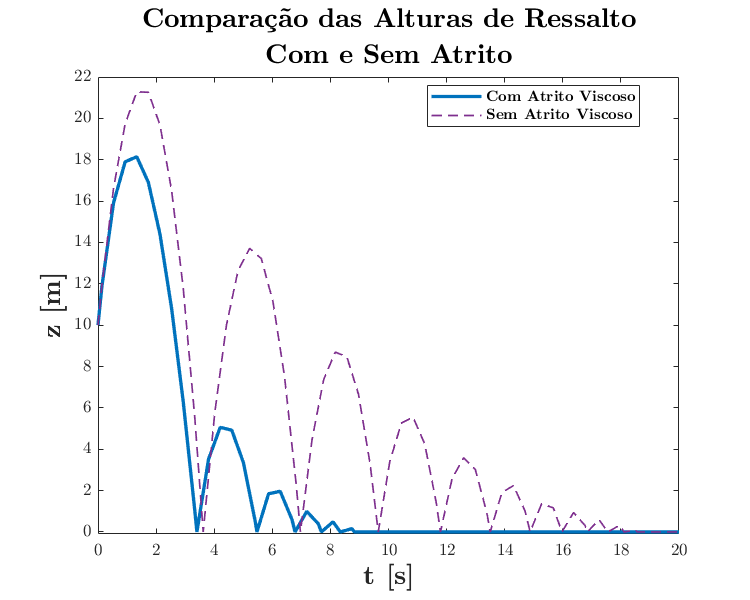
\includegraphics[width=0.6\textwidth]{img/P2/P2-compareTrajetorias.png}
    \caption{Altura de ressalto com efeito do atrito a \textcolor{blue}{azul}.}
    \label{fig:CompareAtrito}
\end{wrapfigure}

\vphantom{123}
\vskip -0.75em
\vphantom{123}

\noindent $\pmb{\rightarrow}$ \textit{\textbf{Observações}}
\\[6pt]
\hspace*{1.2em}$\blacktriangle$ É verificada uma redução da altura máxima que a bola atinge após cada ressalto, face ao exemplo isento de atrito. O fenómeno de Zeno (\textit{vide} \hyperref[subsec:P1]{sec- ção P1})  é também atingido mais rapidamente em relação ao modelo anterior.
\\[6pt]
Esta realidade é trivialmente explicada pela mecânica subja- cente ao problema:

\vskip 3.5em
\noindent $\pmb{\rightarrow}$ \textit{\textbf{Movimento de queda}}

\noindent Reconhecendo que $\dot v_{z_0} = -g \approx -9.81$ ms$^{-2}$, verifica-se um acréscimo de velocidade, subsequentemente, verifica-se um acréscimo de \textit{drag} e um decréscimo da \textit{net force}. Por sua vez o decréscimo da \textit{net force} implica uma redução da velocidade. Deduz-se então que a velocidade continua a crescer, mas cada vez mais lentamente: \underline{A velocidade de impacto é menor na presença de \textit{drag}}.

\vspace{1em}
\noindent $\pmb{\rightarrow}$ \textit{\textbf{Movimento de subida após ressalto}}

\noindent Na subida, para além da velocidade após impacto ser reduzida graças ao efeito de \textit{drag} (a velocidade após impacto é dependente da anterior, \textit{vide} \hyperref[sec:intro]{secção introdutória}), a diminuição da mesma até atingir $v_{z} = 0$ ms$^{-1}$ (onde $z$ atinge $z_\textit{máx}$) é mais veloz, graças à ação da aceleração: ambas as componentes da \textit{net force} apontam na mesma direção (contrária ao movimento): \underline{A altura máxima que a bola atinge após cada ressalto é inferior}.

\clearpage
\noindent $\pmb{\rightarrow}$ \textit{\textbf{Caso Limite: Velocidade Terminal}}

\noindent A velocidade terminal (velocidade constante de queda) é atingida quando $\dot{v}_{z_0} = 0$, consequência da anulação da \textit{net force} onde $F_{drag} = F_g$:
\begin{quote}
    \textit{``Speed continues to increase, but so too does drag. As drag increases, acceleration decreases. Eventually one can imagine a state when the drag and weight forces are equal. You are in equilibrium.''}\cite{elert}
\end{quote}

\noindent Simulando a queda livre da bola\footnotemark[11] de $z_0 = 100$ m e para $\alpha = 1$, o efeito do atrito viscoso, já previamente discutido, é evidente:
\begin{figure}[H]
    \centering
    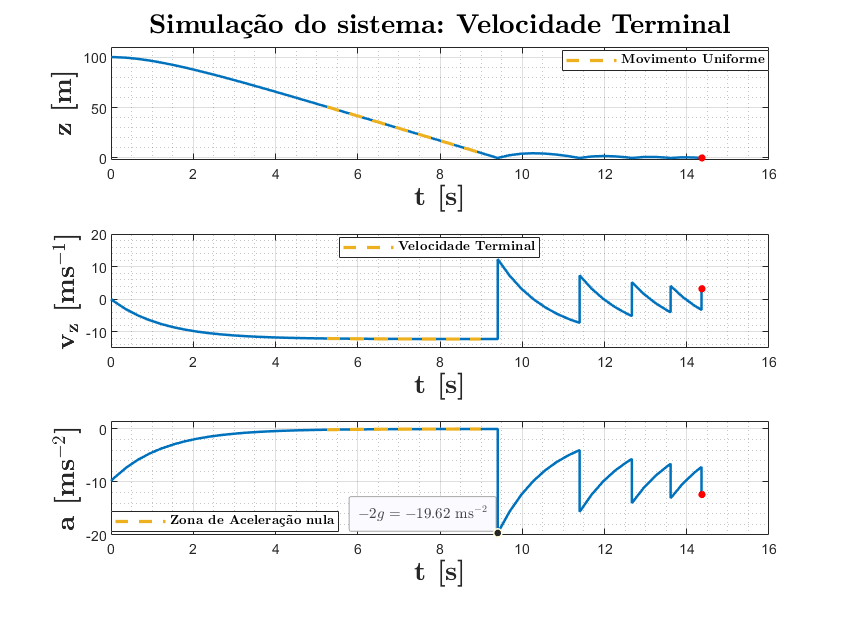
\includegraphics[width = 0.9\linewidth]{img/P2/P2-VelocidadeTerminal.png}
    \caption{Efeito do atrito na aceleração e na velocidade, alcançando a velocidade terminal. O marcador (\textcolor{red}{$\bullet$}) denota o fim da simulação.}
    \label{fig:TerminalVelocity}
\end{figure}

\footnotetext[11]{Em mecânica clássica, a queda livre é o movimento resultante \underline{unicamente} da aceleração provocada pela gravidade (i.e., $v_{z_0} = 0$ ms$^{-1}$).}

\definecolor{MnBlue}{RGB}{60, 79, 118}
\definecolor{LavenderWeb}{RGB}{221, 219, 241}
\setlength\fboxrule{1.5pt}
\hspace*{-1.5em}\fcolorbox{MnBlue}{LavenderWeb}{%
    \minipage[t]{\dimexpr1\linewidth-2\fboxsep-2\fboxrule\relax}
        \noindent $\pmb{\rightarrow}$ \textit{\textbf{Curiosidade}}
        \\
        A aceleração após o impacto é:
        
        \vspace{-0.5em}
        $$
            m\dot v_z = - F_a - mg \implies \dot v_z = - \dfrac{F_{drag}}{m} - g
        $$
        
        \vspace{-0.5em}
        Como a bola atinge a velocidade terminal, sabe-se que:
        $$
            F_{drag} = F_g \implies F_{drag} = mg\; \rightarrow\; \dfrac{F_{drag}}{m} = g
        $$
        
        \vspace{-0.5em}
        Finalmente, resolvendo em ordem a $\dot{v}_z(t_1^+)$, obtém-se:
        $$
            \therefore \dot v_z(t_1^+) = - 2g \rightarrow -19.62 \text{ ms}^{-2}
        $$

        \vspace{-0.5em}
        \hfill\ensuremath{\Box}
    \endminipage}
%//==============================--@--==============================//%
        \clearpage
%//==============================--@--==============================//%
%\vspace{-1em}
\subsection{P3 | Introdução de uma velocidade const. segundo a horizontal}
\label{subsec:P3}

A passagem de uma bola saltitante aliada a um movimento horizontal, entre duas superfícies de impacto distintas, sugere uma alteração ao \textit{jump map} (\textit{vide} \hyperref[sec:intro]{secção introdutória}), no que toca ao coeficiente de restituição aplicado na atualização da velocidade.
$$ 
    \begin{aligned}
         &\mspace{36mu}\textit{\underline{Jump}}\\[-0.7ex]
         &\underbrace{v_z := -\alpha_1 \cdot v_z}_{\text{Superfície 1}}
    \end{aligned}
    \;\xrightarrow[y = 10\text{ m}]{}\;
    \begin{aligned}
         &\mspace{36mu}\textit{\underline{Jump}}\\[-0.7ex]
         &\underbrace{v_z := -\alpha_2 \cdot v_z}_{\text{Superfície 2}}
    \end{aligned}
$$

\iffalse
\noindent Concatenando os \textit{jump maps} para as duas superfícies ao fim de $n$ e $k$ ressaltos obtemos:

$$
    v_z(t_{n+k+1}) = -\alpha_1^{n}\alpha_2^{k} \cdot v_z(t_1)
$$
\fi %rever mais tarde, adoro-te :3

\vspace{1em}
\noindent $\pmb{\rightarrow}$ \textit{\textbf{Velocidade Horizontal}}

\noindent A velocidade horizontal imposta à bola, que governa o seu deslocamento para a direita não sofre qualquer tipo de alteração nem dissipação de energia ao longo de toda a trajetória, já que a aplicação de forças na bola em movimento ocorre somente no eixo vertical, ortogonal à velocidade.
\\\\
A análise da \hyperref[fig:2Pav]{seguinte figura} evidência a diferença entre as perdas energéticas nas respetivas zonas de atenuação para cada impacto:

\begin{figure}[H]
    \centering
    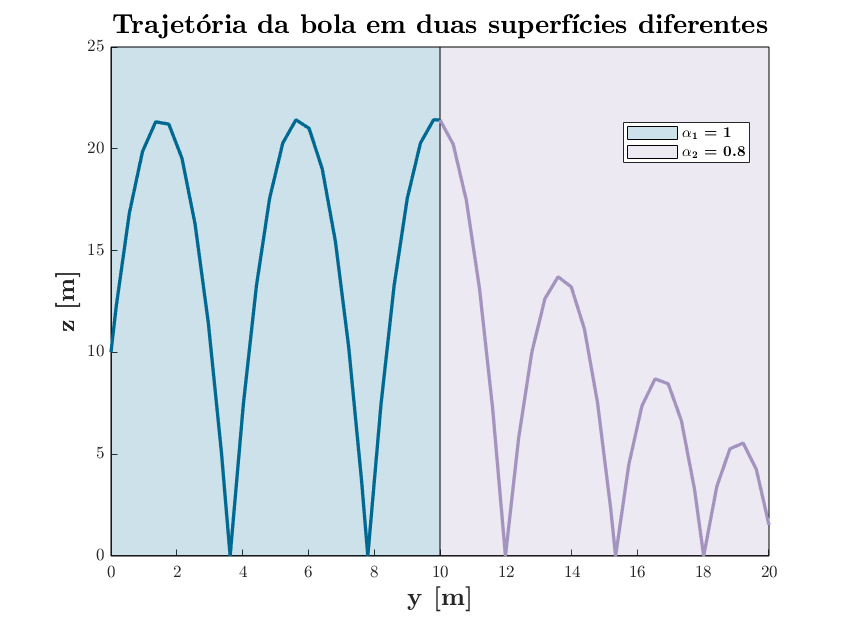
\includegraphics[width = 0.75\linewidth]{img/P3/P3-coefdif.png}
    \caption{Trajetória da bola em duas superfícies distintas com coeficientes de restituição $\alpha_1 = 1$ e $\alpha_2 = 0.8$ e para uma velocidade horizontal constante de $v_y = 1$ ms$^{-1}$ e $v_{z_0} = 15$ ms$^{-1}$.}
    \label{fig:2Pav}
\end{figure}

\noindent\textbf{\textit{$\rightarrow$ Observações}}
\vspace{-0.5em}
\begin{itemize}
    \item[$\blacktriangle$] A passagem da zona de colisão perfeitamente elástica ($\alpha_1 = 1$) para a de $\alpha_2 = 0.8$ verifica uma óbvia diminuição de altura máxima atingida. Como já referido, a atenuação imposta à velocidade vertical sofre uma alteração a partir de $y = 10$ m. Relembrando a discussão realizada na \hyperref[subsec:P1]{secção P1}, um menor coeficiente de restituição contribui para uma maior dissipação de energia a cada impacto, tal equaciona na já mencionada diminuição progressiva de altura comparativamente com a primeira zona de impacto (onde ocorre conservação total de energia $\rightarrow$ não ocorre atenuação da velocidade e consequentemente a altura atingida é sempre a mesma).
    
\end{itemize}
%//==============================--@--==============================//%
        %\clearpage
%//==============================--@--==============================//%
%\vspace{-1em}
\subsection{P4 | Velocidade horizontal constante e choque com uma parede}
\label{subsec:P4}

\noindent De modo a manter a discussão sucinta, apresenta-se um modelo simplificado para a interação da bola saltitante---com velocidade horizontal constante---com superfícies verticais. Não será apresentada uma formulação teórica (tal como na \hyperref[sec:intro]{secção intro- dutória}) para este sistema, pelo que são expostas condições mais relaxadas.

\vspace{-1em}
\begin{figure}[H]
    \centering
    \hspace*{-3.75em}\resizebox{0.8\textwidth}{!}{
        \begin{tikzpicture}[node distance = 2.7cm, on grid, auto, transform shape]
            
            \node[state,
                initial below,
                initial text = {\underline{\texttt{Condições iniciais}}},
                fill=orange!20,
                align=center,
                inner sep=0pt] (q_0) 
            {\textit{\underline{Flow}}\\ $\begin{cases} \dot{z} = v_z\\ \dot{v_z} = -g \\ \dot{y} = v_y\\ \dot{v_y} \equiv 0\end{cases}$};
            
            \path [-stealth, thick]
                (q_0) edge[loop right] 
                node[above, yshift = 0.55cm]
                    {$\begin{aligned}&\mkern-24mu\textit{\underline{Superfície horizontal}} \\ &z \le 0 \land v_z < 0 \end{aligned}$}
                node[right, yshift = -0.25cm] 
                    {$\begin{aligned}
                        &\;\, \textit{\underline{Jump}}\\[-0.7ex]
                        v_z &:= -\alpha_z \cdot v_z
                    \end{aligned}$} 
                (q_0)
    
                (q_0) edge[loop left] 
                node[above, yshift = 0.55cm, xshift = -1.25cm]
                    {$\begin{aligned}&\mkern18mu\textit{\underline{Superfície vertical (paredes)}} \\ (y &\le 0 \land v_y < 0)\lor (y \ge P \land v_y > 0) \end{aligned}$}
                node[left, yshift = -0.25cm] 
                    {$\begin{aligned}
                        &\;\, \textit{\underline{Jump}}\\[-0.7ex]
                        v_y &:= -\alpha_y \cdot v_y
                    \end{aligned}$} 
                (q_0);
                
        \end{tikzpicture}
    }
    \caption{Modelo utilizado computacionalmente do novo sistema híbrido.}
    \label{fig:P4-modelo-computacional-sistema-hibrido}
\end{figure}

\vspace{-1em}
\noindent O modelo simplificado pressupõe \underline{independência entre as componentes ortogonais} da velocidade, i.e., colisões com a superfície horizontal atualizam apenas $v_z$ mediante o valor do coeficiente de restituição da superfície, $\alpha_z$; analogamente, as colisões com a superfície vertical atualizam somente $v_y$ consoante um $\alpha_y$.

%\iffalse
\begin{figure}[H]
    \begin{subfigure}[b]{0.5\linewidth}
        \centering
        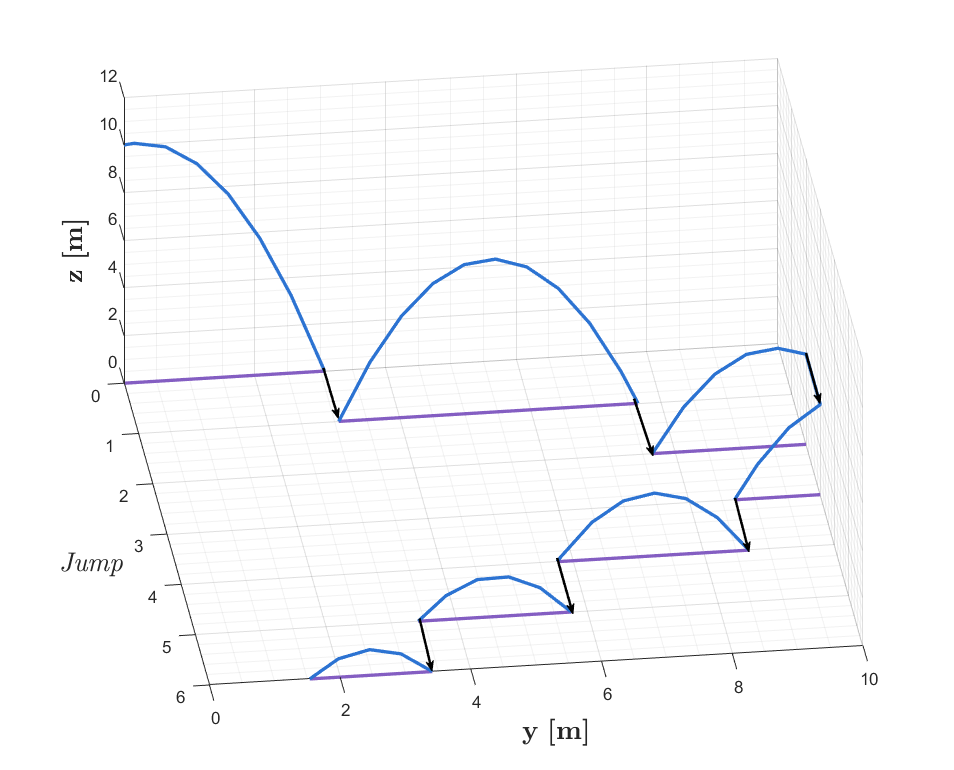
\includegraphics[width=1\linewidth]{img/P4/P4-3dPlot.png}
        \caption{\underline{Trajetória para}:\\ Paredes em $0$ e $P = 10$ m, $z_0 = 10$ m, $v_{z_0} = 0$ ms$^{-1}$, $\alpha_z = 0.8$, $v_y = 2$ ms$^{-1}$ e $\alpha_y = 0.8$.} 
        \label{fig:P4-3dPlot} 
    \end{subfigure}%%
    \begin{subfigure}[b]{0.5\linewidth}
        \centering
        \animategraphics[width=1\textwidth, loop, autoplay]{14}%frame rate
        {img/P4/gif/BouncingBall-}%path to figures
        {0}%start index
        {70}%end index
        \caption{\underline{Trajetória para}:\\ Paredes em $0$ e $P = 5$ m, $z_0 = 10$ m, $v_{z_0} = 30$ ms$^{-1}$, $\alpha_z = 0.8$, $v_y = 2$ ms$^{-1}$ e $\alpha_y = 1$.}
        \label{fig:BouncingBallGif}
    \end{subfigure}%%
    \caption{Visualização da trajetória da massa pontual para duas situações distintas. A \hyperref[fig:BouncingBallGif]{Fig. 11 (b)} é concedida em formato GIF (animada em PDF readers que suportam JavaScript, e.g., Adobe Reader).}
    \label{fig:P4plots}
\end{figure}
%\fi

\vspace{-1em}
\noindent\textbf{\textit{$\rightarrow$ Observações}}
\vspace{-0.5em}
\begin{itemize}
    \item[$\blacktriangle$] A \hyperref[fig:P4-3dPlot]{Fig. 11 (a)} permite vizualizar espacialmente os embates da bola com as super- fícies e os consequentes \textit{jumps} que se sucedem com estes eventos. O resultado final são segmentos da trajetória obtidos com base no período de \textit{flow} que sucede cada \textit{jump}.
    
    \item[$\blacktriangle$] O uso das duas paredes delimita a trajetória da massa puntiforme, como visível na \hyperref[fig:BouncingBallGif]{Fig. 11 (b)}. Esta delimitação permite visualizar com uma maior frequência o efeito da reflexão do movimento horizontal, mantendo a massa pontual \textit{bounded}. Caso não se verificasse \textit{bounded}, a posição tenderia para menos infinito após a primeira colisão com a parede, uma vez que não possui aceleração constante no sentido da superfície vertical em $P$.
\end{itemize}

%//==============================--A--==============================//%
%\clearpage
\noindent De modo a explorar a independendência supramencionada entre as componentes ortogonais do sistemas, é estudada a evolução temporal de cada componente. Para uma melhor visualização, foram selecionados os parâmetros: Paredes em $0$ e $P = 2$ m, $z_0 = 10$ m, $v_{z_0} = 15$ ms$^{-1}$, $\alpha_z = 0.8$, $v_y = 2$ ms$^{-1}$ e $\alpha_y = 0.8$.

%\iffalse
\vspace{-1em}
\begin{figure}[H]
    \begin{subfigure}[b]{0.5\linewidth}
        \centering
        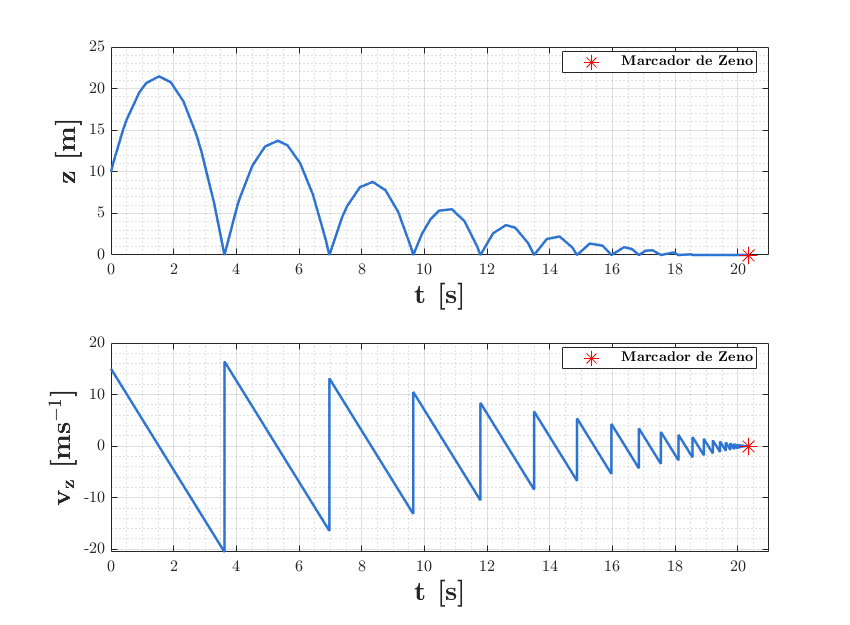
\includegraphics[width=1\linewidth]{img/P4/P4-z}
        \caption{Componente vertical.} 
        \label{fig:P4-z} 
    \end{subfigure}%%
    \begin{subfigure}[b]{0.5\linewidth}
        \centering
        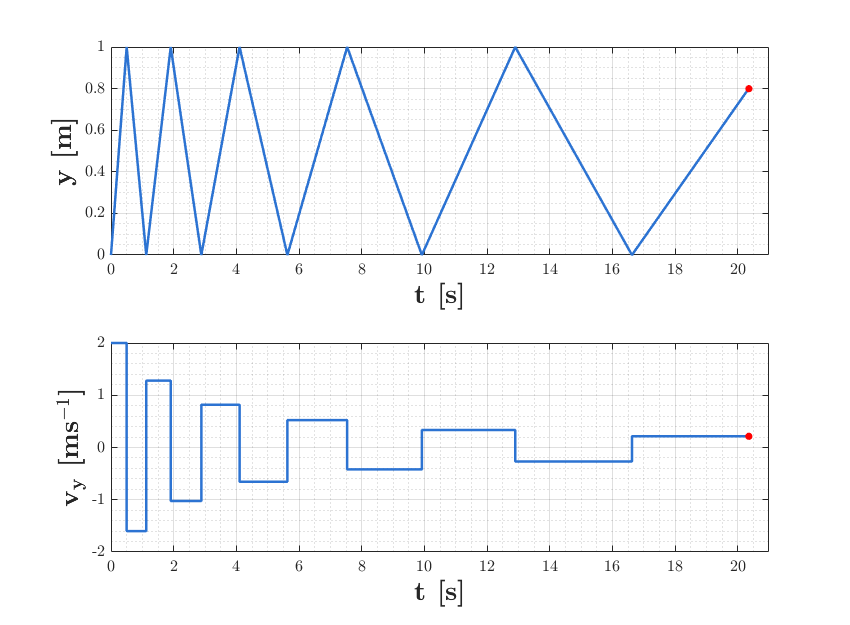
\includegraphics[width=1\linewidth]{img/P4/P4-y}
        \caption{Componente horizontal.} 
        \label{fig:P4-y} 
    \end{subfigure}%%
    \caption{Evolução temporal das componentes verticais e horizontais do sistema. Ao contrário da vertical, os gráficos associados à parte horizontal sofrem uma dilatação ao longo do tempo, dado que as colisões se tornam cada vez menos frequentes, graças à dissipação energética imposta pelo fator $\alpha_y = 0.8$. O marcador (\textcolor{red}{$\bullet$}) denota o fim da simulação (interrompendo o período de \textit{flow}).}
    \label{fig:P4-z-y}
\end{figure}
%\fi

%\iffalse
\vspace{-1.85em}
\begin{figure}[H]
    \begin{subfigure}[b]{0.5\linewidth}
        \centering
        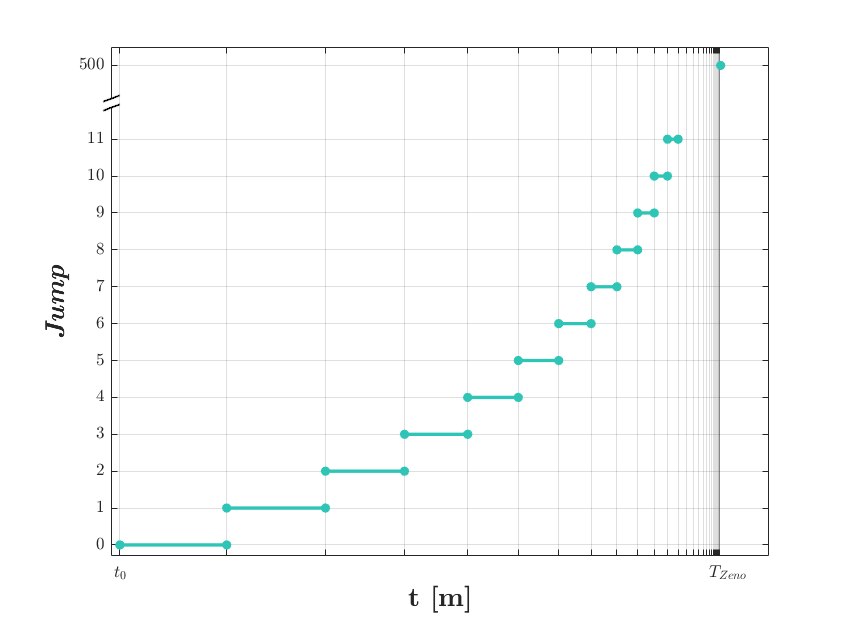
\includegraphics[width=1\linewidth]{img/P4/P4-zeno.png}
        \caption{Componente vertical. Visualização do \hyperref[def:zeno]{efeito de Zeno}. Os intervalos tendem para 0.} 
        \label{fig:P4-zeno} 
    \end{subfigure}%%
    \begin{subfigure}[b]{0.5\linewidth}
        \centering
        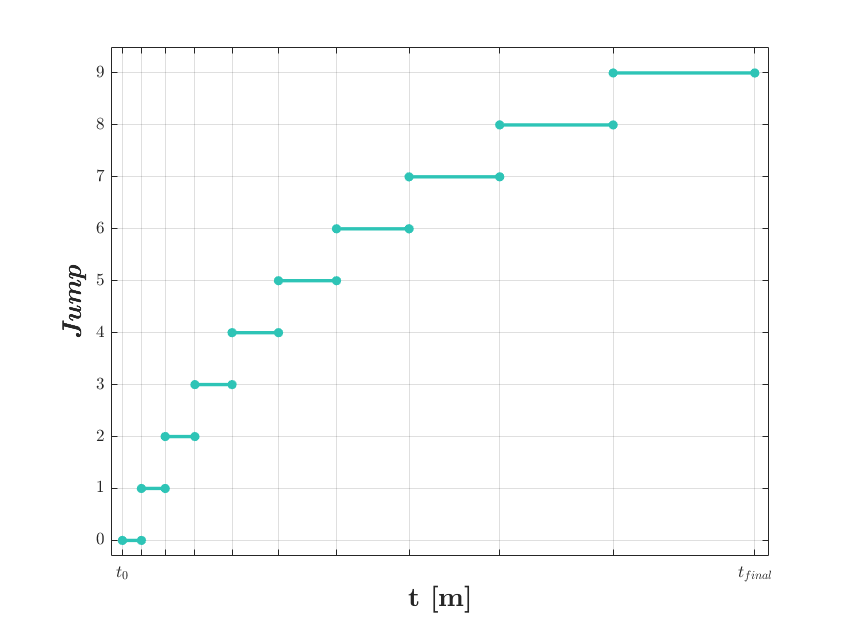
\includegraphics[width=1\linewidth]{img/P4/P4-antizeno.png}
        \caption{Componente horizontal. Efeito da dilatação temporal associada. Os intervalos tendem para infinito.} 
        \label{fig:P4-antizeno} 
    \end{subfigure}%%
    \caption{Evolução da duração dos intervalos de tempo entre colisões com a superfícies horizontal e superfícies verticais. Consoante a discussão na \hyperref[subsec:P1]{secção P1}, verifica-se que $T_{Zeno} =  20.3576$ s, inde- pendente de qualquer influência da componente horizontal, como esperado, dada a ortogonalidade. $t_{final}$ representa o instante final do último período de \textit{flow} completo aparente na \hyperref[fig:P4-y]{Fig. 12 (b)}.}
    \label{fig:P4-zenos}
\end{figure}
%\fi
%//==============================--@--==============================//%
    
    %% refs
    %\clearpage
    \bibliographystyle{unsrtnat}
    \nocite{*}
    {\footnotesize%
    \bibliography{refs}}
    %% attachments
    %\newpage
    %\input{appendix.tex}

\end{document}